\documentclass[12pt]{article}

% -------------------- Packages --------------------
\usepackage{hyperref}
\usepackage{listings}
\usepackage[margin=1in]{geometry}
\usepackage{enumitem}
\usepackage{array}
\usepackage{titlesec}
\usepackage{helvet}
\renewcommand{\familydefault}{\sfdefault}

% Math packages
\usepackage{amsmath}     % For math equations
\usepackage{amssymb}     % For advanced math symbols
\usepackage{amsfonts}    % For math fonts
\usepackage{gvv}         % Custom matrix/vector formatting
\usepackage{esint}

% Other packages
\usepackage[utf8]{inputenc}
\usepackage{graphicx}
\usepackage{pgfplots}
\pgfplotsset{compat=1.18}
\usepackage{multirow}
\usepackage{float}
\usepackage{caption}
\usepackage{multicol}

% -------------------- Formatting --------------------
\titleformat{\section}{\bfseries\large}{\thesection.}{1em}{}
\setlength{\parindent}{0pt}
\setlength{\parskip}{6pt}
\renewcommand{\labelenumi}{\alph{enumi})}

% -------------------- Document --------------------
\begin{document}

\newpage
\begin{center}
\textbf{\Large AI25BTECH11034 - SUJAL CHAUHAN }\\
\textbf{4.4.30}
\end{center}

\textbf{Question:}\\
Show that four points $\vec{A}(4,5,1)$, $\vec{B}(0,-1,-1)$, $\vec{C}(3,9,4)$, $\vec{D}(-4,4,4)$ are coplanar.\\[1cm]

\textbf{Theory:} \\

If $N$ points in $\mathbb{R}^3$ are given as 
\[
X_i = (x_i, y_i, z_i), \quad i = 1,2,\dots,N,
\] 
Let equation of the given plane be 

all four point must satisfy the equation of plane 
\begin{align}
\myvec{\vec{A}&&\vec{B}&&\vec{C} && \vec{D}}=\vec{K}
\end{align}
Now equation will be 
\begin{align}
    \vec{K}^T\vec{n}=\myvec{1 \\ 1\\ 1\\ 1}
\end{align}
making augment matrix which is 

    \begin{align}
 \myvec{
x_1 & y_1 & z_1 & | & 1 \\
x_2 & y_2 & z_2 & | & 1 \\
x_3 & y_3 & z_3 & | & 1 \\
x_4 & y_4 & z_4 & | & 1
} 
\end{align}


then the condition for coplanarity is that the augmented matrix
\begin{align}
A = \myvec{
x_1 & y_1 & z_1 & 1 \\
x_2 & y_2 & z_2 & 1 \\
x_3& y_3 & z_3 & 1 \\
x_4 & y_4 & z_4 & 1
}
\end{align}
satisfies
\begin{align}
\operatorname{rank}(A) \leq 3.
\end{align}



\textbf{Solution:} \\
Equation of plane:
\begin{align}
    \vec{n}^\top\vec{x}=1
\end{align}
Now we have:
Four point which satisfy the plane can be expressed as:
\begin{align}
    \myvec{4 && 5 && 1 \\
           0 && -1 && -1 \\
           3 && 9 && 4 \\
           -4 && 4 && 4 } \vec{n}=\myvec{1 \\ 1 \\ 1 \\1}      
\end{align}
For the given four points to be coplanar, the rank of the following matrix must be less than 4:
\begin{align}
\mathbf{A}=\myvec{ 
4 & 5 & 1 & 1\\
0 & -1 & -1 & 1 \\
3 & 9 & 4 & 1\\
-4 & 4 & 4 & 1 
}
\end{align}

\begin{align}
&\xrightarrow{R_3 \to R_3 - \tfrac{3}{4}R_1,\; R_4 \to R_4 + R_1}
\myvec{
4 & 5 & 1 & 1 \\
0 & -1 & -1 & 1 \\
0 & \tfrac{21}{4} & \tfrac{13}{4} & \tfrac{1}{4} \\
0 & 9 & 5 & 2
}
\end{align}

\begin{align}
&\xrightarrow{R_1 \to \tfrac{1}{4}R_1}
\myvec{
1 & \tfrac{5}{4} & \tfrac{1}{4} & \tfrac{1}{4} \\
0 & -1 & -1 & 1 \\
0 & \tfrac{21}{4} & \tfrac{13}{4} & \tfrac{1}{4} \\
0 & 9 & 5 & 2
}
\end{align}

\begin{align}
&\xrightarrow{R_2 \to -R_2}
\myvec{
1 & \tfrac{5}{4} & \tfrac{1}{4} & \tfrac{1}{4} \\
0 & 1 & 1 & -1 \\
0 & \tfrac{21}{4} & \tfrac{13}{4} & \tfrac{1}{4} \\
0 & 9 & 5 & 2
}
\end{align}

\begin{align}
&\xrightarrow{R_3 \to R_3 - \tfrac{21}{4}R_2,\; R_4 \to R_4 - 9R_2}
\myvec{
1 & \tfrac{5}{4} & \tfrac{1}{4} & \tfrac{1}{4} \\
0 & 1 & 1 & -1 \\
0 & 0 & -2 & \tfrac{22}{4} \\
0 & 0 & -4 & 11
}
\end{align}

\begin{align}
&\xrightarrow{R_3 \to -\tfrac{1}{2}R_3}
\myvec{
1 & \tfrac{5}{4} & \tfrac{1}{4} & \tfrac{1}{4} \\
0 & 1 & 1 & -1 \\
0 & 0 & 1 & -\tfrac{11}{4} \\
0 & 0 & -4 & 11
}
\end{align}

\begin{align}
&\xrightarrow{R_4 \to R_4 + 4R_3}
\myvec{
1 & \tfrac{5}{4} & \tfrac{1}{4} & \tfrac{1}{4} \\
0 & 1 & 1 & -1 \\
0 & 0 & 1 & -\tfrac{11}{4} \\
0 & 0 & 0 & 0
}
\end{align}

Thus,
\begin{align}
\operatorname{rank}(\mathbf{A}) = 3 \;<\; 4 \;\;\implies\;\;
\text{The given points are coplanar.}
\end{align}

\newpage
\begin{figure}[H]
    \centering
    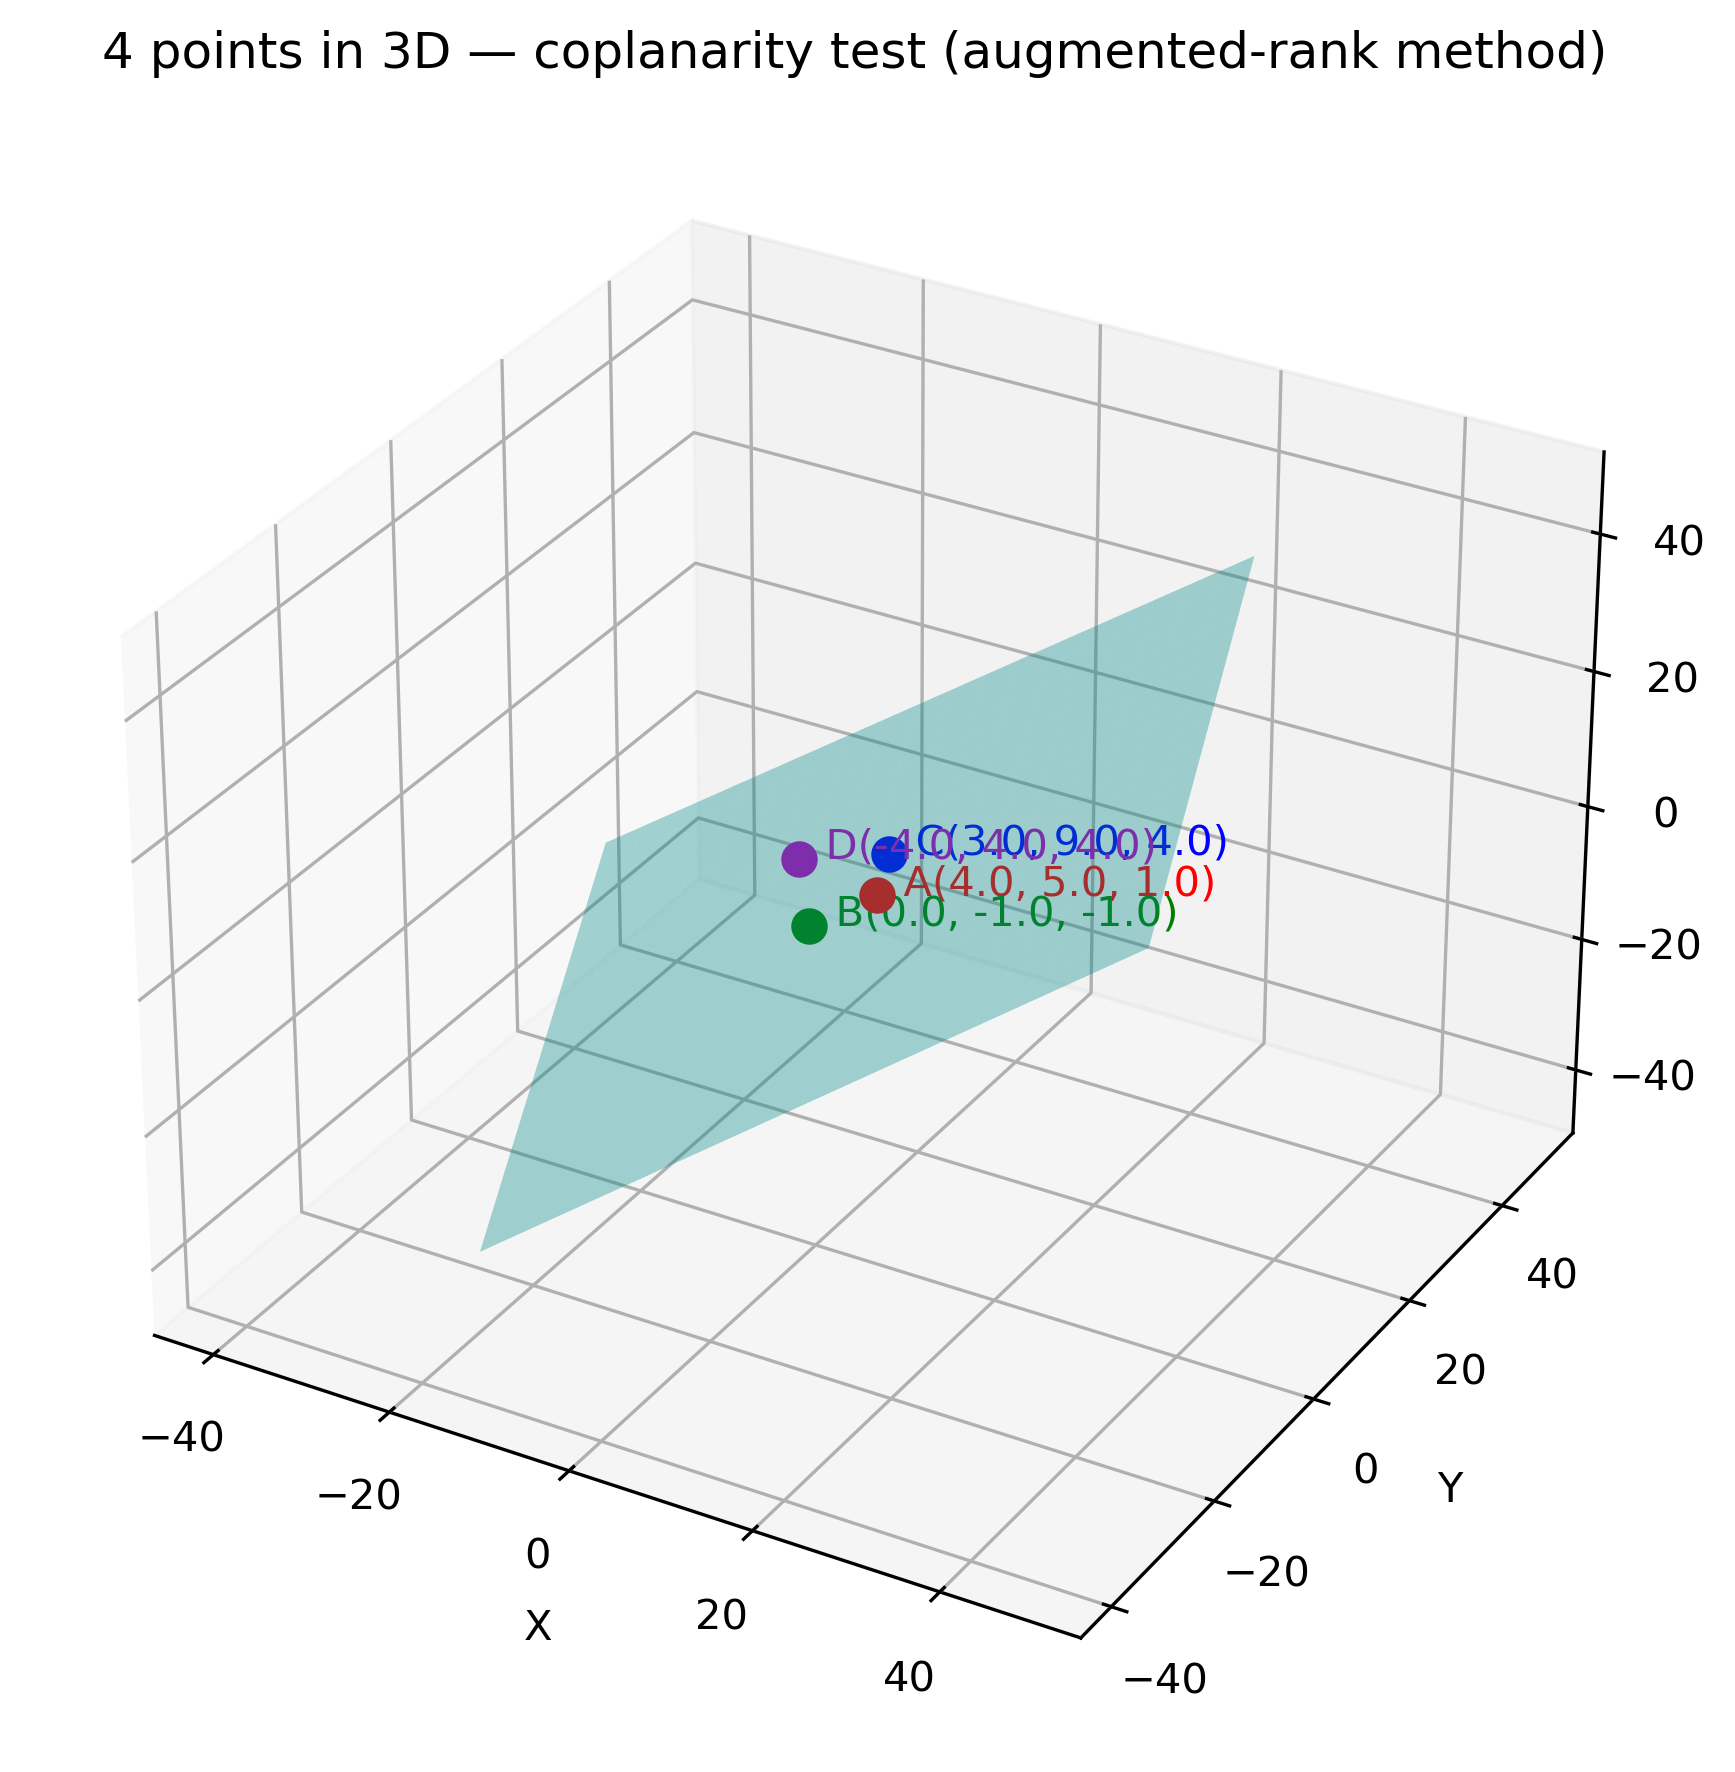
\includegraphics[width=0.55\linewidth]{figures/points_coplanarity.png}
    \caption{Geometric visualization of points $A, B, C, D$ lying on the same plane.}
    \label{fig:coplanarity}
\end{figure}

\end{document}

